\documentclass[11pt]{article}

\usepackage[letterpaper, bottom=2cm, right=2cm]{geometry}
\geometry{margin=2cm}

\usepackage{amssymb,amsmath,amsthm} % Símbolos matemáticos
\usepackage[english]{babel}
\usepackage[utf8]{inputenc} % Acentos y otros símbolos 
\usepackage{enumerate}

\usepackage{graphicx}
\DeclareGraphicsExtensions{.pdf}
\pdfcompresslevel=9  % Maximum compression
\pdfobjcompresslevel=3

\usepackage{placeins}
\usepackage{booktabs}
\usepackage{etoolbox}
\usepackage{bbm}
\usepackage{tocloft}
\usepackage{etoc}
\usepackage{setspace}
\usepackage{caption}
\usepackage{subcaption}
\usepackage{ifdraft}
\usepackage{comment}
\usepackage{lscape}
\usepackage{pdfcomment}

\usepackage[looser]{newpxtext} % LOOSER = BETTER WORD SPACE

%\AtBeginEnvironment{table}{\scriptsize}
\AtEndEnvironment{table}{\vspace{0.2in}}

\AtEndEnvironment{figure}{\vspace{0.2in}}

% Para eliminar guiones y justificar texto
\tolerance=1
\emergencystretch=\maxdimen
\hyphenpenalty=10000
\hbadness=10000

\linespread{1.5} 

\let\oldfootnote\footnote % Deja espacio entre el número del pie de página y el inicio del texto
\renewcommand\footnote[1]{%
\oldfootnote{\hspace{0.05mm}#1}}

\renewcommand{\thefootnote} {\textcolor{black}{\arabic{footnote}}} % Súperindice a color negro

\setlength{\footnotesep}{0.75\baselineskip} % Espaciado entre notas al pie

\usepackage{fnpos} % Footnotes al final de pág.

\usepackage[justification=centering, font=bf, labelsep=period, skip=5pt]{caption} % Centrar captions de tablas y ponerlas en negritas
\usepackage{subcaption}

\usepackage{tabularx} % Big tables
\usepackage{multirow}
\usepackage{adjustbox}
\usepackage{longtable}
\usepackage{lscape}

\usepackage{float} % Float tables

\usepackage{color, soul}
\usepackage[dvipsnames]{xcolor} % Color
% Define Maroon color
\definecolor{Maroon}{RGB}{128,0,0}

\usepackage{natbib}
\bibliographystyle{aer}
\setcitestyle{authoryear,aysep={},yysep={,}}
%\setcitestyle{authoryear,open={(},close={)}} %Citation-related commands
\renewcommand{\bibsection}{\section*{References}}

\usepackage{pgfplots} % Gráficas
\pgfplotsset{compat=newest}
\pgfplotsset{width=7.5cm}
\pgfkeys{/pgf/number format/1000 sep={}}

\usepackage{tgpagella}
\usepackage[T1]{fontenc}

\addto\captionsspanish{
    \renewcommand*{\contentsname}{Contents}
    }

\newcommand{\expectation}{\mathbb{E}}
\newcommand{\indicator}{\mathbbm{1}}
\newcommand{\bluetext}[1]{\textcolor{blue}{#1}}

%Added by Roberto for to do notes
\usepackage{marginnote}
\renewcommand*{\marginfont}{\color{red}\sffamily}
\usepackage[colorinlistoftodos]{todonotes}
%\setuptodonotes{fancyline, color=yellow}

\newcommand{\smalltodo}[2][]
{\todo[caption={#2}, #1]
{\begin{spacing}{0.5}#2\end{spacing}}}
%\setlength{\marginparwidth}{2cm}

% https://mirror.hmc.edu/ctan/macros/latex/contrib/todonotes/todonotes.pdf
\newcounter{todoListItems}
\newcommand{\todoLink}[2][ ]{
% Increment counter
\addtocounter{todoListItems}{1}
\todo[%
caption={\protect\hypertarget{todo\thetodoListItems}{}Translation},
#1]
{
#2 \hfill
\hyperlink{todo\thetodoListItems}{$\uparrow$}
}
}

\newcommand{\td}{\todoLink}
\newcommand{\forMW}[1]{\td[color=green!20,inline,caption={\thetodoListItems:
    For @Maria}]{\textbf{@Maria} -- #1}}
\newcommand{\forRG}[1]{\td[color=blue!20,inline,caption={\thetodoListItems:
    For @Roberto}]{\textbf{@Roberto} -- #1}}
\newcommand{\forES}[1]{\td[color=red!20,inline,caption={\thetodoListItems:
    For @Enrique}]{\textbf{@Enrique} -- #1}}
\newcommand{\forAll}[1]{\td[color=orange!20,inline,caption={\thetodoListItems:
    For All}]{\textbf{@All} -- #1}}

\newcommand{\notes}[1]{\footnotesize{#1}}

\definecolor{ultramarine}{RGB}{4,55,242}

\definecolor{LinkBlue}{RGB}{0,35,200}

% For capitalizing first letter referencing sections
\addto\extrasenglish{
    \def\sectionautorefname{Section}
}
 
\usepackage{hyperref} % Hipervínculos en el índice

% Set up configurations for hyperreferences
\hypersetup{colorlinks=true, breaklinks=true, citecolor=Maroon, linkcolor=LinkBlue, menucolor=Maroon, urlcolor=Maroon}

% -----------------------------------------------------------------------
% Focused version of the paper.  Same arguments and framing as
% violent-effects-of-apex-corruption-main.tex, but the body evidence is a
% curated set: Table 1; the pooled (Pres+Other Apex) vs Other Non-Apex
% test; four subsample event studies; the football/depreciation benchmark
% table (with shares); and the 2008-democracy split.  Self-contained (no
% appendix); shares the same preamble, figures, tables and refs.bib.
% -----------------------------------------------------------------------

% (1) Where to look for figures / tables produced by the Stata pipeline.
\graphicspath{{../../Protest_Work/results/figures/}{./figures/}}
\makeatletter
\providecommand*{\input@path}{}
\edef\input@path{{../../Protest_Work/results/tables/}{./tables/}\input@path}
\makeatother

% (2) Allow PDF figures up to v1.7 (Stata exports v1.6).
\pdfminorversion=7

% (3) Allow .png event-study figures alongside .pdf.
\DeclareGraphicsExtensions{.pdf,.png}

% (4) Wrap \beta with \ensuremath so esttab's exp(\beta) resolves.
\let\mathbetasym\beta
\renewcommand{\beta}{\ensuremath{\mathbetasym}}

% -----------------------------------------------------------------------

\title{\bfseries\Large Apex Corruption causes Violent Protests\thanks{We thank seminar audiences and colleagues for helpful comments. All errors are our own.}}

\author{%
Roberto Gonz\'alez-T\'ellez\thanks{Research Fellow, Stanford Graduate School of Business. \texttt{rob98@stanford.edu}}  \and Saumitra Jha\thanks{Stanford Graduate School of Business. \texttt{saumitra@stanford.edu}.}
\and
Eduardo Rivera\thanks{MIT, Department of Economics. \texttt{erivera@mit.edu}.} \and
Enrique Seira\thanks{University of Notre Dame, Department of Economics and Kellogg Institute. \texttt{eseirabe@nd.edu}.}
%
}

\date{This draft: \today}

\begin{document}

\maketitle

% =====================================================================
% ABSTRACT
% =====================================================================
\begin{abstract}
    \noindent We document that \textit{apex} corruption scandals---corrupt acts implicating top-level politicians---cause immediate and persistent increases in violent protests. Using a panel of 176 corruption scandals across 23 countries in Latin America from 2008 to 2018, merged with daily protest counts, we show that the daily count of violent protests rises sharply after scandals implicating a President or Other Apex official---by about 0.06 protests per country-day in the month following disclosure, roughly 1.7 times the pre-scandal baseline---while scandals implicating non-apex officials produce no such immediate response, and a pooled test rejects equality of the two effects. The response appears within a week of disclosure and persists even in a four month window. It is specific to apex corruption: neither football match losses nor currency depreciations, two other high-salience national shocks, move violent protests. Our findings identify a high-frequency, high-magnitude channel through which corruption shapes the political environment in democracies.
\end{abstract}

% \noindent \textbf{Keywords:} \\
% \textbf{JEL Code:}

\bigskip

% =====================================================================
% INTRODUCTION
% =====================================================================
\clearpage
\section{Introduction}

Political violence is among the most consequential outcomes a democracy can experience. Civil unrest disrupts economic activity, displaces investment, and---when met with state violence in return---erodes the social contract that legitimizes the regime. An influential economic literature has linked political violence to economic shocks~\citep{miguel2004economic,mcguirk2020economic}, to commodity rents and network structure~\citep{koenig2017networks,dube2013commodity}, to the foundations of state capacity~\citep{besley2011logic}, and in recent work to abrupt withdrawals of foreign assistance~\citep{rohner2026aidingpeace}. Related work shows that protests themselves can produce durable political effects~\citep{madestam2013protests,bursztyn2021persistent}. The contribution of political shocks to events that change citizens' beliefs about who governs them, however, has received considerably less attention. In this paper we argue that disclosures of apex corruption are one such shock, and that the behavioral consequences for political violence are large, immediate, and persistent.

Corruption has been long studied, with known costs for growth and public goods provision~\citep{mauro1995corruption,treisman2007what,olken2007monitoring,olken2012corruption,glaeser2006corruption}. In the past two decades, citizens' perceptions of corruption prevalence have risen~\citep{cantoni2024protests}, and corruption scandals associated to \textit{apex} politicians have drawn more attention from news outlets in recent years~\citep{ApexCorruption}; perhaps unsurprisingly due to the expansion of social media, which reduces the cost of diffusing information and enables news outlets to reach broader audiences \citep{enikolopov2018SocialMedia, tufekci2024twitter,dellavigna2007fox}. Even though exposing corruption scandals on news outlets can have positive desired effects, such as political accountability or crackdowns of corruption networks \citep{ferraz2011electoral, horacio2019infonetwork, horacio2022metaketa}, it can also have negative undesired effects on democratic values \citep{ajzenman2021powerexample, ApexCorruption} and away from the polling booths. Public exposure of malfeasance by sitting officials changes what citizens believe about who governs them and about the rules under which the government operates. The most consequential corruption-related political moments of the last decade, such as Brazil's Lava Jato\footnote{See \href{https://www.youtube.com/watch?v=boK0Mh2T5nk}{this video} for more information on the scandal.}, were mobilization events, not electoral ones.

We document that apex corruption---corrupt acts implicating top-level politicians---triggers immediate and persistent increases in violent protests. Using a hand-curated panel of 176 corruption scandals across 23 Latin American countries from 2008 to 2018, merged with daily protest counts from the Mass Mobilization (MM) project~\citep{clark2016mass}, we establish four facts. First, the daily count of violent protests rises sharply following scandals implicating a President or Other Apex official, while the count of peaceful protests is largely unaffected; scandals implicating Congressmen, lower judiciary, and other non-apex officials leave protest patterns broadly unchanged, and we can reject that the two effects are equal. Second, the effect appears within a week of disclosure and the point estimate remains positive even four months later, with no evidence of pre-trends. Third, the response is specific to apex corruption: neither national-team football losses~\citep[see e.g.,][]{DuranteFutbol} nor currency depreciations---two other high-salience, plausibly as-good-as-randomly-timed national shocks---move violent protests. Fourth, exploring heterogeneity by the 2008 level of democracy, the response is present across countries and, if anything, somewhat larger and more persistent in higher-democracy countries, though the high- versus low-democracy difference is not statistically significant.

% =====================================================================
% Method
% =====================================================================
\section{Method}\label{sec:methods}
\subsection{Study Design and Measures}

Our empirical analyses exploit the randomness of corruption scandal disclosures in Latin American news outlets between 2008 and 2018. In particular, we use an interrupted time-series design in which we compare protest occurrences in countries with scandals before and after the scandal occurs. Our analysis dataset is created by: (i) Scraping the Twitter accounts from news outlets in Latin America to identify the calendar date in which a scandal in a given country is first reported\footnote{We keep the date of the first news report to (a) be able to estimate the effect of a scoop, and (b) avoid double-counting a scandal due to follow-up news reports on it.}, (ii) create an event-window of $T \in \{30, 120\}$ days before and after the scandal, (iii) merge the country-day count of protests from the MM data to create a `scandal-protest' dataset for a given country in a given calendar-date window, and lastly, (iv) append all such scandal-protest datasets to build the analysis dataset.

The MM dataset is available for the period 1990--2020, and it includes information on the date, size, and location of any episode in which 50 or more protesters publicly demonstrate against the State. If a protest lasts $X$ days, we code the occurrence of a protest at date $t, t+1, \dots, t+X-1$. If the same protest is associated with more than one date (e.g., because the news source for the protest cannot accurately identify whether it is a continued or a new protest), then we keep the date of the earliest protest. For a protest to be classified as ``violent'', ``[t]he violence could include anything from riotous behavior that destroys property to shooting at the police or military''~\citep{clark2016mass}. Our main outcome is the number of protests occurring in a given country-date. We focus on the years 2008--2018, given that our corruption scandals data is available for those years.

Importantly, our recolection of scandals allows us to identify the position of the implicated politician. We then look at the scandals and manually classify them in three categories: (i) ``President'' includes scandals in which the implicated official is a President (current or former), (ii) ``Other Apex'' includes scandals in which the implicated official is either a Governor or Supreme Court Justice, and (iii) ``Other Non-Apex'' includes scandals in which the implicated official is a Congressman, lower judiciary, or other lower-rank officials. Throughout, we group the President and Other Apex scandals together (``apex''; 64 scandals) and contrast them with the Other Non-Apex scandals (112 scandals).

We use Ordinary Least Squares (OLS) to estimate the following equation on each of our Apex and Non-Apex samples:
\begin{equation}
\label{eq:main}
    Y_{c(s)t} = \beta \; \mathbbm{1}\{t \geq \text{Scandal Date}_{c(s)}\} + \alpha_{d} + \lambda_{m} + \theta_{cy} + \varepsilon_{c(s)t}
\end{equation}
where $\alpha_d$ denote day of the week fixed effects, $\lambda_m$ denote month of the year fixed effects, $\theta_{cy}$ denote country-year fixed effects, $\text{Scandal Date}_{c(s)}$ is the date in which corruption scandal $s$ in country $c$ occurs, $Y_{ct}$ denotes the outcome of interest in country $c$ at date $t$, and $\varepsilon_{c(s)t}$ is an idiosyncratic error term.

To trace dynamics we replace $\mathbbm{1}\{t \geq \text{Scandal Date}_{c(s)}\}$ in \autoref{eq:main} with a saturated set of 30-day bin indicators for four months before/after the scandal.  The reference category in each time-to-event graph is the bin immediately before disclosure (i.e., $w_{s,t} \in [-30, -1]$).

The identification assumption we rely on for our estimates to be interpreted as causal is that conditional on country-year, month-of-year, and day-of-week fixed effects, the within-year date of disclosure of a scandal is as-good-as-randomly assigned in relation to the protest baseline of the country. The country-year fixed effects absorb every source of country-year-level confounding such as pre-existing political instability, electoral calendars, or institutional reforms. The day-of-week and month-of-year fixed effects absorb weekly and seasonal cycles in protest activity.

% =====================================================================
% Results
% =====================================================================
\section{Results}

\subsection{Apex corruption increases violent protests}

\autoref{tab:main} reports OLS estimates of the post-scandal effect on violent and peaceful protests, split by the political rank of the implicated official. Panel A restricts the sample to Apex scandals; Panel B restricts to Other Non-Apex scandals. Each panel reports eight outcome--window cells: violent and peaceful protest \emph{counts} on the $\pm$30- and $\pm$120-day windows, and the corresponding violent/peaceful \emph{shares}\footnote{We define the share outcomes at the country-day level by dividing the number of violent (peaceful) protests by the total protests, and impute a 0 if there are no protests in a given day. Given tha there is only one protest in most cases for country-days in which there is mobilization, our outcomes are highly correlated and the corresponding estimates are very similar.}. The contrast is stark. In the President + Other Apex panel, the daily count of violent protests rises by 0.060 per country-day in the $\pm$30-day window ($p<0.01$)---about 1.7 times the pre-scandal baseline of 0.036---and by 0.021 in the $\pm$120-day window ($p<0.1$). In the Other Non-Apex panel the immediate ($\pm$30-day) violent effect is essentially zero (0.000), with only a smaller, delayed increase of 0.016 at the $\pm$120-day horizon ($p<0.05$). Strikingly, peaceful protests move little in either panel at either horizon.

\begin{table}[htb!]
    \caption{Violent protests increase after apex corruption scandal disclosures.}
    \label{tab:main}
    \begin{center}
        \scriptsize{{
\def\sym#1{\ifmmode^{#1}\else\(^{#1}\)\fi}
\begin{tabular}{l*{8}{c}}
\toprule
&\multicolumn{2}{c}{$\pm 30$-Day Window}    &\multicolumn{2}{c}{$\pm 120$-Day Window}   &\multicolumn{2}{c}{Shares ($\pm 30$-Day)}  &\multicolumn{2}{c}{Shares ($\pm 120$-Day)} \\\cmidrule(lr){2-3}\cmidrule(lr){4-5}\cmidrule(lr){6-7}\cmidrule(lr){8-9}
&\multicolumn{1}{c}{(1)}&\multicolumn{1}{c}{(2)}&\multicolumn{1}{c}{(3)}&\multicolumn{1}{c}{(4)}&\multicolumn{1}{c}{(5)}&\multicolumn{1}{c}{(6)}&\multicolumn{1}{c}{(7)}&\multicolumn{1}{c}{(8)}\\
&\multicolumn{1}{c}{\shortstack{Violent\\Protests}}&\multicolumn{1}{c}{\shortstack{Peaceful\\Protests}}&\multicolumn{1}{c}{\shortstack{Violent\\Protests}}&\multicolumn{1}{c}{\shortstack{Peaceful\\Protests}}&\multicolumn{1}{c}{\shortstack{Share\\Violent}}&\multicolumn{1}{c}{\shortstack{Share\\Peaceful}}&\multicolumn{1}{c}{\shortstack{Share\\Violent}}&\multicolumn{1}{c}{\shortstack{Share\\Peaceful}}\\
\midrule \multicolumn{9}{l}{\textbf{\textit{Panel A: President + Other Apex}}} \\
Post Scandal&       0.055\sym{***}&       0.005         &       0.015         &       0.002         &       0.055\sym{***}&       0.004         &       0.015         &      -0.001         \\
&     (0.016)         &     (0.009)         &     (0.013)         &     (0.010)         &     (0.016)         &     (0.008)         &     (0.013)         &     (0.009)         \\
\midrule
Mean (Pre-Scandal Bin)&       0.037         &       0.019         &       0.028         &       0.015         &       0.037         &       0.019         &       0.027         &       0.014         \\
Observations&        3843         &        3843         &       15424         &       15424         &        3843         &        3843         &       15424         &       15424         \\
Number of Scandals&          63         &          63         &          63         &          63         &          63         &          63         &          63         &          63         \\
R-squared   &       0.290         &       0.076         &       0.208         &       0.118         &       0.296         &       0.082         &       0.212         &       0.116         \\
\midrule
\multicolumn{9}{l}{\textbf{\textit{Panel B: Other Non-Apex}}} \\
Post Scandal&      -0.000         &       0.010         &       0.016\sym{**} &      -0.010         &      -0.001         &       0.012         &       0.016\sym{**} &      -0.010         \\
&     (0.005)         &     (0.010)         &     (0.008)         &     (0.009)         &     (0.005)         &     (0.011)         &     (0.008)         &     (0.009)         \\
\midrule
Mean (Pre-Scandal Bin)&       0.022         &       0.097         &       0.017         &       0.075         &       0.022         &       0.084         &       0.016         &       0.067         \\
Observations&        6893         &        6893         &       27233         &       27233         &        6893         &        6893         &       27233         &       27233         \\
Number of Scandals&         113         &         113         &         113         &         113         &         113         &         113         &         113         &         113         \\
R-squared   &       0.113         &       0.564         &       0.106         &       0.358         &       0.122         &       0.577         &       0.109         &       0.349         \\
\midrule
Country $\times$ Year FE&  \checkmark         &  \checkmark         &  \checkmark         &  \checkmark         &  \checkmark         &  \checkmark         &  \checkmark         &  \checkmark         \\
\bottomrule
\end{tabular}
}
}
    \end{center}
    \footnotesize{OLS estimates of $\beta$ from \autoref{eq:main}, split by the political rank of the implicated official. Panel A restricts the sample to scandals implicating a sitting President or an Other Apex official (Governors and Supreme Court Justices; 64 scandals); Panel B restricts to Other Non-Apex scandals (Congressmen, lower judiciary, and other officials; 112 scandals). Each panel reports eight outcome--window combinations: violent and peaceful protest \emph{counts} on the $\pm$30-day window (columns 1--2) and the $\pm$120-day window (columns 3--4); and \emph{share} outcomes---the fraction of the country-day's protests that are violent or peaceful (country-days with no protests imputed to a share of 0)---on the $\pm$30-day window (columns 5--6) and the $\pm$120-day window (columns 7--8). An observation is a country-day inside the event window of a scandal in the corresponding subsample. All specifications include country-by-year, month-of-year, and day-of-week fixed effects; standard errors (in parentheses) are clustered at the country $\times$ year $\times$ day-bin level. ``Mean (Pre-Scandal Bin)'' is the average outcome in the bin immediately before disclosure (a 6-day bin in columns 1--2 and 5--6, a 30-day bin in columns 3--4 and 7--8). Sample period 2008--2018; Venezuela excluded. Significance: $^{*}$ $p<0.1$, $^{**}$ $p<0.05$, $^{***}$ $p<0.01$.}
\end{table}

To make the Apex-vs-Non-Apex contrast explicit, \autoref{tab:interaction} pools the two subsamples into a single specification and formally tests whether the post-scandal effect differs between them. For each outcome and window we estimate
\begin{equation*}
    Y_{c(s)t} \;=\; \beta_{\text{Apex}}\, \mathrm{Post}_{st}\, \mathbf{1}\{\text{Apex}_s\}
    \;+\; \beta_{\text{NA}}\, \mathrm{Post}_{st}\, \mathbf{1}\{\text{Non-Apex}_s\}
    \;+\; \alpha_d + \lambda_m + \theta_{cy} + \varepsilon_{c(s)t},
\end{equation*}
where $\mathrm{Apex}_s$ ($\mathrm{Non-Apex}_s$) indicates a President + Other Apex (Other Non-Apex) scandal, and the row ``$p$-value: Pres+Other Apex $=$ Other Non-Apex'' reports the two-sided $p$-value for $H_0:\beta_{\text{Apex}}=\beta_{\text{Non-Apex}}$. In this pooled specification the immediate ($\pm$30-day) violent-protest effect is 0.048 for apex scandals ($p<0.01$) versus $-0.003$ for non-apex scandals, and we reject equality of the two ($p = 0.020$). At the $\pm$120-day horizon both are positive (0.022 for apex, $p<0.05$; 0.012 for non-apex), though they are no longer statistically distinguishable ($p = 0.411$). The \emph{immediate} violent response to corruption is thus concentrated among apex scandals.

\begin{table}[htb!]
    \caption{Apex scandals cause violent mobilization while Non-Apex scandals do not.}
    \label{tab:interaction}
    \begin{center}
        \scriptsize{{
\def\sym#1{\ifmmode^{#1}\else\(^{#1}\)\fi}
\begin{tabular}{l*{6}{c}}
\toprule
            &\multicolumn{2}{c}{$\pm 30$-Day Window}    &\multicolumn{2}{c}{$\pm 60$-Day Window}    &\multicolumn{2}{c}{$\pm 90$-Day Window}    \\\cmidrule(lr){2-3}\cmidrule(lr){4-5}\cmidrule(lr){6-7}
            &\multicolumn{1}{c}{(1)}&\multicolumn{1}{c}{(2)}&\multicolumn{1}{c}{(3)}&\multicolumn{1}{c}{(4)}&\multicolumn{1}{c}{(5)}&\multicolumn{1}{c}{(6)}\\
            &\multicolumn{1}{c}{\shortstack{Violent\\Protests}}&\multicolumn{1}{c}{\shortstack{Peaceful\\Protests}}&\multicolumn{1}{c}{\shortstack{Violent\\Protests}}&\multicolumn{1}{c}{\shortstack{Peaceful\\Protests}}&\multicolumn{1}{c}{\shortstack{Violent\\Protests}}&\multicolumn{1}{c}{\shortstack{Peaceful\\Protests}}\\
\midrule
Post $\times$ Apex&       0.051\sym{***}&      -0.007         &       0.040\sym{***}&      -0.008         &       0.026\sym{**} &      -0.005         \\
            &     (0.019)         &     (0.013)         &     (0.014)         &     (0.009)         &     (0.011)         &     (0.009)         \\
Post $\times$ Non-Apex&      -0.006         &       0.019         &       0.003         &       0.006         &       0.002         &      -0.002         \\
            &     (0.008)         &     (0.013)         &     (0.007)         &     (0.013)         &     (0.006)         &     (0.010)         \\
\midrule
p-value: Apex $=$ Non-Apex&       0.021         &       0.236         &       0.040         &       0.402         &       0.062         &       0.824         \\
p-value: Apex $>$ Non-Apex (one-sided)&       0.011         &       0.882         &       0.020         &       0.799         &       0.031         &       0.588         \\
Mean (Pre-Scandal)&       0.020         &       0.053         &       0.021         &       0.056         &       0.024         &       0.057         \\
Observations&       10614         &       10614         &       21054         &       21054         &       31494         &       31494         \\
Number of Scandals&         174         &         174         &         174         &         174         &         174         &         174         \\
R-squared   &       0.176         &       0.479         &       0.162         &       0.398         &       0.137         &       0.349         \\
\bottomrule
\end{tabular}
}
}
    \end{center}
    \footnotesize{OLS estimates of $\beta_{\text{Apex}}$ and $\beta_{\text{Non-Apex}}$ from the pooled specification above, on the same eight outcome--window cells as Table~\ref{tab:main}. The row ``$p$-value: Pres+Other Apex $=$ Other Non-Apex'' reports the two-sided $p$-value for $H_0:\beta_{\text{Apex}}=\beta_{\text{Non-Apex}}$. Standard errors in parentheses are clustered at the country $\times$ year $\times$ day-bin level. Same fixed effects and sample period as Table~\ref{tab:main}. Significance: $^{*}$ $p<0.1$, $^{**}$ $p<0.05$, $^{***}$ $p<0.01$.}
\end{table}

\subsection{Protest dynamics around apex corruption scandals}

\autoref{fig:dynamics} traces the dynamics of the effect, replacing the post-scandal indicator with a fully saturated set of 30-day event-time bin indicators over the $\pm 120$-day window,  andestimated separately on the two subsamples of Table~\ref{tab:main}. In the Apex subsample, violent protests (\autoref{fig:dynamics:pav}) show arguably no pre-trend and then jump at disclosure, remaining elevated in the month that follows before converging back to the pre-scandal levels; peaceful protests (\autoref{fig:dynamics:pap}) show no immediate increase, but they do however slightly increase in the months that follow, though by a small magnitude. In the Non-Apex subsample, violent protests (\autoref{fig:dynamics:nav}) do not increase by large amounts with scandal disclosures, and the response is delayed. Overall, Non-Apex scandals cause no effects---positive or negative---on peaceful protests (\autoref{fig:dynamics:nap}). The absence of a pre-trend in every panel supports the identifying assumption that the within-year timing of disclosure is as good as random relative to the protest baseline.

\begin{figure}[htb!]
    \caption{Protest dynamics by apex-partition subsample ($\pm 120$-day window, 30-day bins).}
    \label{fig:dynamics}
    \begin{center}
    \begin{subfigure}{0.45\textwidth}
        \caption{Violent, President + Other Apex.}
        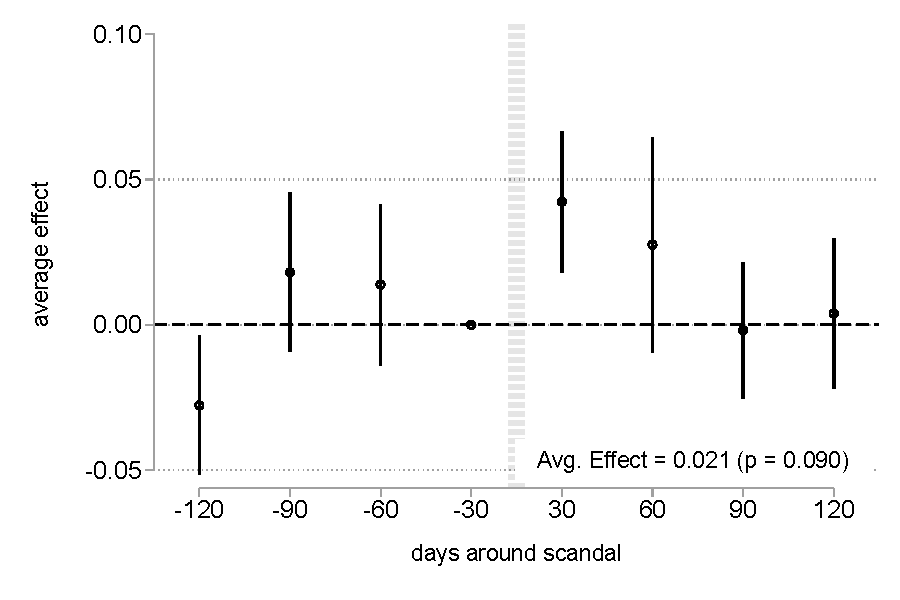
\includegraphics[width=\textwidth]{es_num_violent_MM_120d_pa_ols_90ci.pdf}
        \label{fig:dynamics:pav}
    \end{subfigure}\hfill
    \begin{subfigure}{0.45\textwidth}
        \caption{Peaceful, President + Other Apex.}
        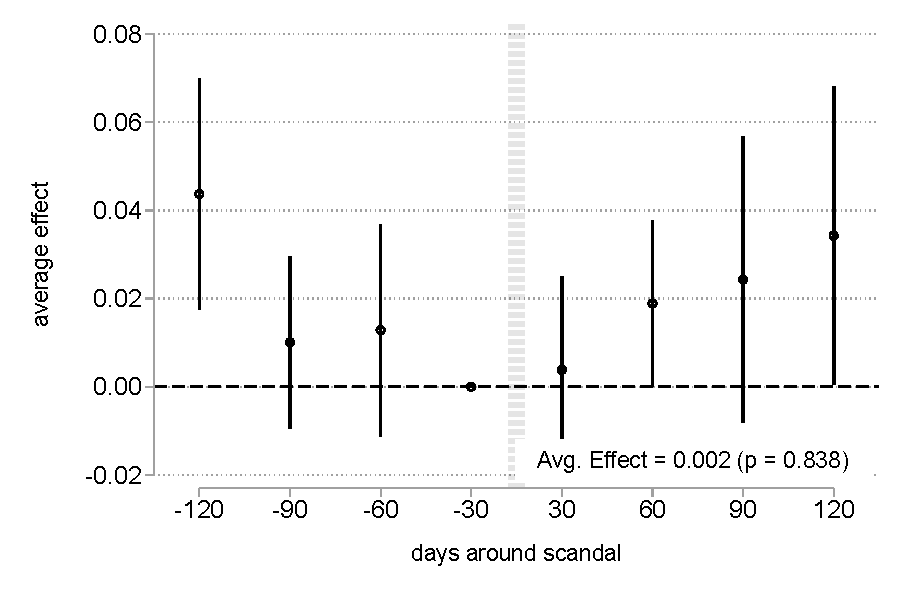
\includegraphics[width=\textwidth]{es_num_peaceful_MM_120d_pa_ols_90ci.pdf}
        \label{fig:dynamics:pap}
    \end{subfigure} \\
    \begin{subfigure}{0.45\textwidth}
        \caption{Violent, Other Non-Apex.}
        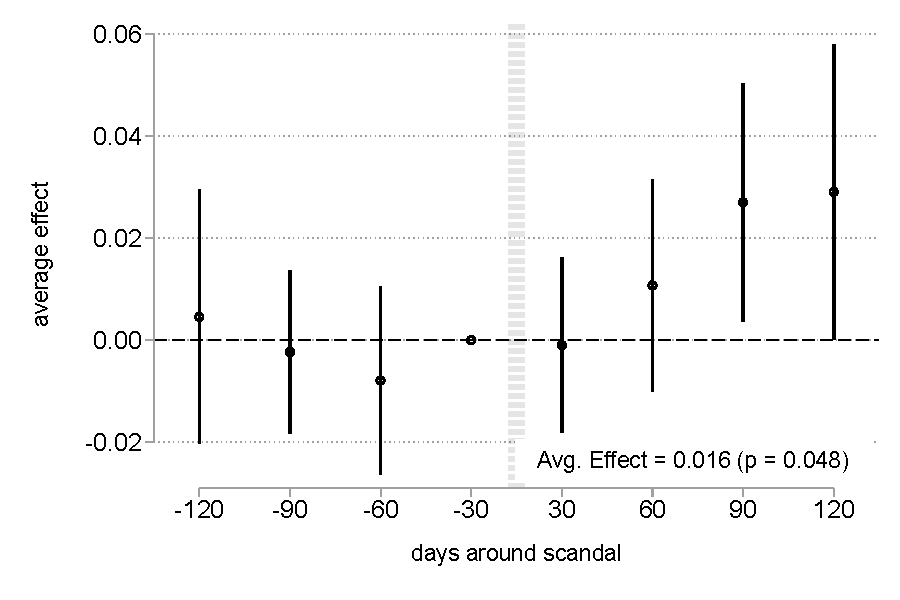
\includegraphics[width=\textwidth]{es_num_violent_MM_120d_na_ols_90ci.pdf}
        \label{fig:dynamics:nav}
    \end{subfigure}\hfill
    \begin{subfigure}{0.45\textwidth}
        \caption{Peaceful, Other Non-Apex.}
        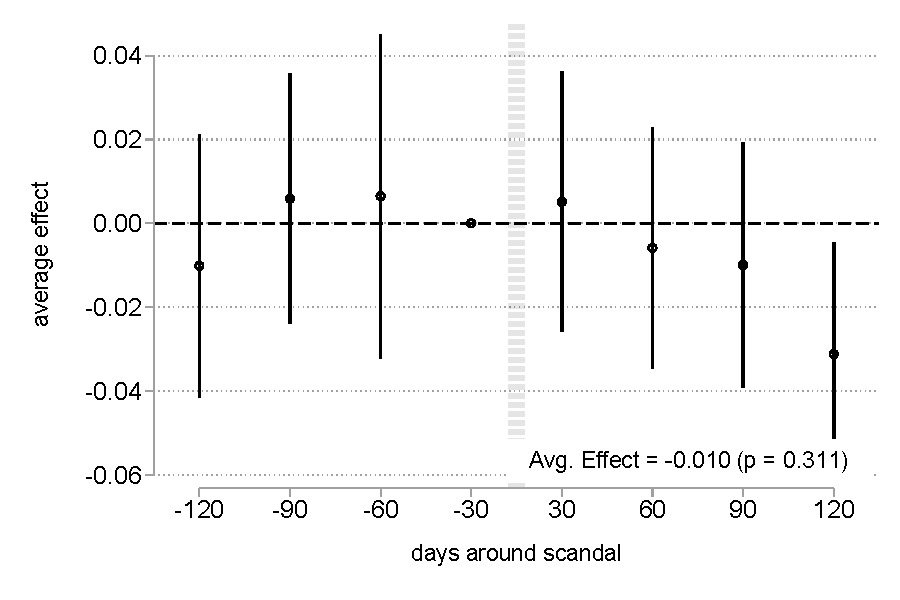
\includegraphics[width=\textwidth]{es_num_peaceful_MM_120d_na_ols_90ci.pdf}
        \label{fig:dynamics:nap}
    \end{subfigure}
    \end{center}
    \footnotesize{OLS estimates on event-time 30-day-bin indicators from the modified \autoref{eq:main}, estimated separately on the President + Other Apex subsample (top row) and the Other Non-Apex subsample (bottom row). The omitted reference bin is the 30 days immediately preceding the scandal ($w_{s,t}\in[-30,-1]$). Vertical bars are 90\% confidence intervals; standard errors clustered at country $\times$ year $\times$ day-bin. An observation is a country-scandal-date. Sample period 2008--2018; Venezuela excluded.}
\end{figure}

\subsection{The protest response is specific to apex corruption}

Is the violent-protest response a general reaction to salient national news, or is it specific to apex corruption? To answer this question, \autoref{tab:benchmarks} benchmarks the corruption effect against two other high-salience national shocks whose timing is plausibly as-good-as-random with respect to the protest baseline: national-team football (soccer) match losses and currency depreciation episodes. Each shock is estimated using \autoref{eq:main} and the same eight outcome--window columns (counts and shares), but changing the post-scandal indicator for an indicator of a national football team loss, or a month-to-month depreciation of the exchange rate of more than 5\%. The table reproduces Panels A and B of \autoref{tab:main} so that both headline corruption regressions can be read directly against the two benchmarks. The apex-corruption effect on violent protests in the $\pm$30-day window (0.060, $p<0.01$) is an order of magnitude larger than---and statistically unlike---the corresponding football (0.006) and currency-depreciation (0.004) estimates, neither of which is distinguishable from zero. The mobilization response is thus specific to apex corruption, not a generic reaction to salient national events.

\begin{table}[htb!]
    \caption{Benchmarking the corruption effect against football losses and currency depreciations.}
    \label{tab:benchmarks}
    \begin{center}
        \scriptsize{{
\def\sym#1{\ifmmode^{#1}\else\(^{#1}\)\fi}
\begin{tabular}{l*{8}{c}}
\toprule
&\multicolumn{2}{c}{$\pm 30$-Day Window}    &\multicolumn{2}{c}{$\pm 120$-Day Window}   &\multicolumn{2}{c}{Shares ($\pm 30$-Day)}  &\multicolumn{2}{c}{Shares ($\pm 120$-Day)} \\\cmidrule(lr){2-3}\cmidrule(lr){4-5}\cmidrule(lr){6-7}\cmidrule(lr){8-9}
&\multicolumn{1}{c}{(1)}&\multicolumn{1}{c}{(2)}&\multicolumn{1}{c}{(3)}&\multicolumn{1}{c}{(4)}&\multicolumn{1}{c}{(5)}&\multicolumn{1}{c}{(6)}&\multicolumn{1}{c}{(7)}&\multicolumn{1}{c}{(8)}\\
&\multicolumn{1}{c}{\shortstack{Violent\\Protests}}&\multicolumn{1}{c}{\shortstack{Peaceful\\Protests}}&\multicolumn{1}{c}{\shortstack{Violent\\Protests}}&\multicolumn{1}{c}{\shortstack{Peaceful\\Protests}}&\multicolumn{1}{c}{\shortstack{Share\\Violent}}&\multicolumn{1}{c}{\shortstack{Share\\Peaceful}}&\multicolumn{1}{c}{\shortstack{Share\\Violent}}&\multicolumn{1}{c}{\shortstack{Share\\Peaceful}}\\
\midrule \multicolumn{9}{l}{\textbf{\textit{Panel A: Apex corruption (President + Other Apex)}}} \\
Post Event  &       0.060\sym{***}&       0.005         &       0.021\sym{*}  &       0.002         &       0.060\sym{***}&       0.005         &       0.021\sym{*}  &      -0.000         \\
&     (0.017)         &     (0.008)         &     (0.012)         &     (0.010)         &     (0.017)         &     (0.008)         &     (0.012)         &     (0.009)         \\
\midrule
Mean (Pre-Event Bin)&       0.036         &       0.018         &       0.027         &       0.015         &       0.036         &       0.018         &       0.027         &       0.014         \\
Observations&        3904         &        3904         &       15665         &       15665         &        3904         &        3904         &       15665         &       15665         \\
Number of Events&          64         &          64         &          64         &          64         &          64         &          64         &          64         &          64         \\
R-squared   &       0.270         &       0.075         &       0.193         &       0.117         &       0.275         &       0.081         &       0.197         &       0.116         \\
\midrule
\multicolumn{9}{l}{\textbf{\textit{Panel B: Non-apex corruption (Other Non-Apex)}}} \\
Post Event  &       0.000         &       0.010         &       0.016\sym{**} &      -0.010         &      -0.001         &       0.012         &       0.016\sym{**} &      -0.010         \\
&     (0.005)         &     (0.010)         &     (0.008)         &     (0.009)         &     (0.005)         &     (0.011)         &     (0.008)         &     (0.009)         \\
\midrule
Mean (Pre-Event Bin)&       0.022         &       0.098         &       0.017         &       0.075         &       0.022         &       0.085         &       0.016         &       0.068         \\
Observations&        6832         &        6832         &       26992         &       26992         &        6832         &        6832         &       26992         &       26992         \\
Number of Events&         112         &         112         &         112         &         112         &         112         &         112         &         112         &         112         \\
R-squared   &       0.115         &       0.565         &       0.107         &       0.358         &       0.124         &       0.578         &       0.109         &       0.349         \\
\bottomrule
\multicolumn{9}{l}{\textbf{\textit{Panel C: Football match losses}}} \\
Post Event  &       0.006         &       0.002         &       0.002         &       0.013         &       0.006         &       0.004         &       0.004         &       0.014         \\
&     (0.005)         &     (0.012)         &     (0.006)         &     (0.014)         &     (0.005)         &     (0.012)         &     (0.006)         &     (0.014)         \\
\midrule
Mean (Pre-Event Bin)&       0.006         &       0.042         &       0.009         &       0.043         &       0.006         &       0.041         &       0.008         &       0.040         \\
Observations&       10004         &       10004         &       39524         &       39524         &       10004         &       10004         &       39524         &       39524         \\
Number of Events&         164         &         164         &         164         &         164         &         164         &         164         &         164         &         164         \\
R-squared   &       0.674         &       0.598         &       0.431         &       0.295         &       0.680         &       0.594         &       0.417         &       0.293         \\
\bottomrule
\multicolumn{9}{l}{\textbf{\textit{Panel D: Currency depreciations}}} \\
Post Event  &       0.004         &      -0.003         &      -0.007         &      -0.013\sym{**} &       0.004         &      -0.003         &      -0.005         &      -0.013\sym{**} \\
&     (0.010)         &     (0.008)         &     (0.006)         &     (0.006)         &     (0.010)         &     (0.008)         &     (0.005)         &     (0.005)         \\
\midrule
Mean (Pre-Event Bin)&       0.020         &       0.028         &       0.025         &       0.027         &       0.019         &       0.026         &       0.024         &       0.027         \\
Observations&        9638         &        9638         &       38064         &       38064         &        9638         &        9638         &       38064         &       38064         \\
Number of Events&         158         &         158         &         158         &         158         &         158         &         158         &         158         &         158         \\
R-squared   &       0.331         &       0.275         &       0.361         &       0.123         &       0.340         &       0.280         &       0.357         &       0.117         \\
\bottomrule
\end{tabular}
}
}
    \end{center}
    \footnotesize{OLS estimates of $\beta$ from \autoref{eq:main} on the same eight outcome--window cells as Table~\ref{tab:main}. Panel A: apex corruption scandals (President + Other Apex); Panel B: non-apex corruption scandals (Other Non-Apex); Panel C: national-team football match losses; Panel D: currency depreciation episodes. All panels share the same country-by-year, month-of-year and day-of-week fixed effects and cluster at country $\times$ year $\times$ day-bin. ``Mean (Pre-Event Bin)'' is the average outcome in the 6-day ($\pm$30) or 30-day ($\pm$120) bin immediately preceding the event. Sample period 2008--2018; Venezuela excluded. Significance: $^{*}$ $p<0.1$, $^{**}$ $p<0.05$, $^{***}$ $p<0.01$.}
\end{table}

\subsection{Heterogeneity by the level of democracy}

A natural question is whether these patterns of mobilization are driven by the country's democratic environment. There are at least two related, yet opposite, hypotheses about how democratic level of a country interacts with mobilization patterns. On the one hand, citizens in countries with higher levels of democracy may not mobilize, since strong democratic institutions in their countries can punish corrupt officials and remove them from office once proven guilty. On the other hand, precisely because citizens in highly democratic countries have higher standards for accountability, they may choose to mobilize in order to call democratic institutions into action. Our evidence suggests this second behavior is more likely the explanation. 

\autoref{tab:democracy} splits the panel of countries at the median of their 2008 level of democracy---measured by V-Dem's Electoral Democracy Index~\citep{vdem2024}---and interacts the post-scandal indicator with the resulting above-/below-median classification. The violent-protest response is positive in both groups but, if anything, larger and more persistent in the \emph{above}-median (higher-democracy) countries: the $\pm$30-day effect is 0.021 ($p<0.05$) in higher-democracy countries versus 0.009 ($p<0.1$) in lower-democracy ones, and at the $\pm$120-day horizon it is 0.024 ($p<0.01$) versus 0.005 (not significant). However, we cannot statistically distinguish the two ($p = 0.245$ and $0.115$ for the $\pm$30- and $\pm$120-day violent-count effects), so this heterogeneity is suggestive rather than conclusive.

\begin{table}[htb!]
    \caption{Effect by 2008 level of democracy.}
    \label{tab:democracy}
    \begin{center}
        \scriptsize{{
\def\sym#1{\ifmmode^{#1}\else\(^{#1}\)\fi}
\begin{tabular}{l*{6}{c}}
\toprule
            &\multicolumn{2}{c}{$\pm 30$-Day Window}    &\multicolumn{2}{c}{$\pm 60$-Day Window}    &\multicolumn{2}{c}{$\pm 90$-Day Window}    \\\cmidrule(lr){2-3}\cmidrule(lr){4-5}\cmidrule(lr){6-7}
            &\multicolumn{1}{c}{(1)}&\multicolumn{1}{c}{(2)}&\multicolumn{1}{c}{(3)}&\multicolumn{1}{c}{(4)}&\multicolumn{1}{c}{(5)}&\multicolumn{1}{c}{(6)}\\
            &\multicolumn{1}{c}{\shortstack{Violent\\Protests}}&\multicolumn{1}{c}{\shortstack{Peaceful\\Protests}}&\multicolumn{1}{c}{\shortstack{Violent\\Protests}}&\multicolumn{1}{c}{\shortstack{Peaceful\\Protests}}&\multicolumn{1}{c}{\shortstack{Violent\\Protests}}&\multicolumn{1}{c}{\shortstack{Peaceful\\Protests}}\\
\midrule
Post $\times$ High Democracy (2008)&       0.018\sym{**} &       0.013         &       0.022\sym{**} &       0.003         &       0.016\sym{*}  &      -0.004         \\
            &     (0.008)         &     (0.008)         &     (0.010)         &     (0.009)         &     (0.009)         &     (0.008)         \\
Post $\times$ Low Democracy (2008)&       0.010\sym{*}  &       0.006         &       0.010\sym{*}  &      -0.001         &       0.005         &      -0.002         \\
            &     (0.005)         &     (0.012)         &     (0.005)         &     (0.016)         &     (0.007)         &     (0.013)         \\
\midrule
p-value: High $=$ Low&       0.396         &       0.583         &       0.311         &       0.827         &       0.352         &       0.875         \\
Mean (Pre-Scandal)&       0.020         &       0.053         &       0.021         &       0.056         &       0.024         &       0.057         \\
Observations&       10614         &       10614         &       21054         &       21054         &       31494         &       31494         \\
Number of Scandals&         174         &         174         &         174         &         174         &         174         &         174         \\
R-squared   &       0.164         &       0.478         &       0.158         &       0.398         &       0.136         &       0.349         \\
\bottomrule
\end{tabular}
}
}
    \end{center}
    \footnotesize{OLS estimates of $\beta_{\text{High}}$ and $\beta_{\text{Low}}$ (Post $\times$ above-/at-or-below-median 2008 democracy) on the same eight outcome--window cells as Table~\ref{tab:main}. Countries are split at the median of V-Dem's \texttt{v2x\_polyarchy} in 2008 (16 panel countries; Venezuela excluded). The row ``$p$-value: High $=$ Low'' tests $H_0:\beta_{\text{High}}=\beta_{\text{Low}}$. Same fixed effects, clustering, and sample as Table~\ref{tab:main}. Significance: $^{*}$ $p<0.1$, $^{**}$ $p<0.05$, $^{***}$ $p<0.01$.}
\end{table}

% =====================================================================
% Discussion
% =====================================================================
\section{Discussion}
The evidence we have presented suggests citizens do not respond uniformly to all types of corruption: they respond sharply, immediately and durably when the implicated official is at the apex of the political spectrum, and they barely respond when the implicated official sits at the lower tier of the hierarchy. Furthermore, the response concentrates on violent protests and persists even in a four month window. The peaceful margin stays essentially flat over both horizons and regardless of whether the scandal implicates an Apex or Non-Apex politician. Our findings underscore the fact that corruption is a tangible behavioral shock to the local (and perhaps even regional) political environment, not just an attitudinal one. The stakes citizens hold in the continuation in office of a corrupt official appear to govern whether citizens mobilize, and how they do so. The joint pattern---a persistent rise in violent protests with no corresponding change on the peaceful margin---is consistent with, though our design does not establish, citizens turning to violent rather than peaceful channels when a scandal undercuts their confidence in the officials meant to be held accountable.

Our findings contribute to three literatures. First, the economics-of-conflict literature has documented that political violence responds to economic shocks~\citep{koenig2017networks,mcguirk2020economic,dube2013commodity,besley2011logic,berman2011hearts,rohner2026aidingpeace}. We introduce a \textit{political} shock---public disclosure of apex corruption---and show that it produces mobilization responses of comparable magnitude to the ones caused by economic shocks. Second, the corruption and accountability literature has documented that disclosures of malfeasance change voting behavior~\citep{ferraz2008exposing,ferraz2011electoral,FerrazFinanAccount,ferraz2018audits,horacio2019infonetwork}. The slow electoral horizon has tended to obscure that the same disclosures can have very fast, non-electoral consequences~\citep{madestam2013protests,bursztyn2021persistent}. Our high-frequency design uncovers a channel through which apex corruption shapes the political environment in democracies within days of public disclosures, well before subsequent elections come into play. Third, the protest channel is the behavioral complement of the attitudinal evidence from our companion paper~\citep{ApexCorruption}, which documents that apex corruption scandals erode support for democracy and democratic institutions, and also reduce political participation.

Our results help reconcile part of the mixed results in the existing literature on the political consequences of corruption disclosures. Studies of local level corruption have produced muted estimates of disclosure's electoral consequences, with some finding modest accountability gains in Brazil and Spain~\citep{ferraz2008exposing,ferraz2011electoral,ferraz2018audits,costasperez2012corruption} and others finding null or even demobilizing effects~\citep{chong2015does,anduiza2013turning,pavao2018corruption,horacio2022metaketa}. We argue that the dispersion in municipal estimates reflects the limited political stakes at that level. In particular, when the implicated official is one of many municipal officeholders, citizens have weaker incentives to incur the costs of mobilization. Within our sample, scandals implicating Congressmen, lower judiciary and lower rank officials have \emph{immediate} (30-day) post-scandal effects on violent protests statistically indistinguishable from zero, whereas the effect of scandals implicating a President or Other Apex official is large and immediate.

A ``salience of stakeholders'' view rationalizes this~\citep{acemoglu2006origins,acemoglu2012nations,jha2013trade,jha2019valuing,jha2022markets}. Citizens' political behavior responds to the political weight of \textit{what} is being disclosed. Apex corruption, thus, affects citizens' perceived stakes of the political bargain, particularly when the implicated official is at the apex of the political hierarchy. The contrast between high--stakes apex scandals and low-stakes lower-officials scandals parallels the contrast between high-stakes elections and routine governance in studies of political accountability~\citep{martinezbravo2022elites}. Notably, this response does not require weak institutions to appear: it is present across our sample and, if anything, somewhat stronger in the more democratic countries, where citizens plausibly hold higher expectations of accountability---and enjoy greater latitude to voice them---when those expectations are violated~\citep{acemoglu2019DemoEcoGrowth,acemoglu2024demobreedsupport,DuranteFutbol}.

Our empirical analyses have some limitations worth noting. Our identification strategy relies on the timing of apex corruption disclosures, not on the timing of the corrupt act itself. If the timing of disclosures is correlated with pre-existing political conditions that affect mobilization (violent or peaceful), our estimates could then be biased. Somewhat reassuringly, the pre-scandal estimates in \autoref{fig:dynamics} show no evidence of pre-existing trends in mobilization. A second limitation comes from the fact that the MM dataset is constructed by looking at news sources reporting on mobilization events. Small protests may thus be underreported as they are not big enough to draw media attention, or protests occurring in geographically remote areas may also be left out. This would induce measurement error in our estimates, but if anything this would bias our estimates toward zero. And finally, our scandal sample is limited to Latin American democracies in the 2008--2018 period, thus limiting the external validity of our findings insofar as different regions in the world may mobilize differently in response to corruption scandals. One could also expect different results when shortening/expanding the time scope of the analysis if one believes that the cumulative amount of apex corruption episodes affect the extent to which citizens mobilize.

% =====================================================================
% REFERENCES
% =====================================================================
\clearpage
\bibliography{refs}

% =====================================================================
% SUPPLEMENTARY MATERIALS
% =====================================================================
\clearpage
\appendix
\renewcommand{\thesection}{S\arabic{section}}
\renewcommand{\thesubsection}{S\arabic{section}.\arabic{subsection}}
\renewcommand{\thetable}{S\arabic{table}}
\renewcommand{\thefigure}{S\arabic{figure}}
\setcounter{section}{0}
\setcounter{table}{0}
\setcounter{figure}{0}

\begin{center}
    {\Large\bfseries Supplementary Materials}
\end{center}
\bigskip

% ---------------------------------------------------------------------
\clearpage
\section{Randomization inference by apex-partition subsample}\label{sup:ri}

We complement the headline estimates with a randomization-inference (permutation) test, run separately on the two subsamples of Table~\ref{tab:main}. In each of 1{,}000 replications and for each scandal we draw a placebo disclosure date uniformly at random within the scandal's original country-year, rejecting any draw whose $\pm T$-day window would overlap a real disclosure date in the same country (with an unconditional fallback over all countries and 2008--2018 dates after 20 failed within-country-year attempts). We rebuild the $\pm T$-day event-window panel around the accepted placebo dates and re-estimate the headline OLS specification. Figures~\ref{fig:sup_ri_pa} and \ref{fig:sup_ri_na} plot the resulting placebo $\hat\beta$ distributions; the maroon vertical line marks the observed $\hat\beta$ from the corresponding cell of Table~\ref{tab:main}, and the legend reports the two-sided randomization-inference $p$-value. For violent protests the observed effect sits in the upper tail---most sharply for the President + Other Apex subsample---while for the Other Non-Apex subsample and for peaceful protests it lies within the placebo mass.

\begin{figure}[htb!]
    \caption{Randomization inference on the President + Other Apex subsample.}
    \label{fig:sup_ri_pa}
    \begin{subfigure}{0.48\textwidth}
        \caption{Violent protests, $\pm 30$-day window.}
        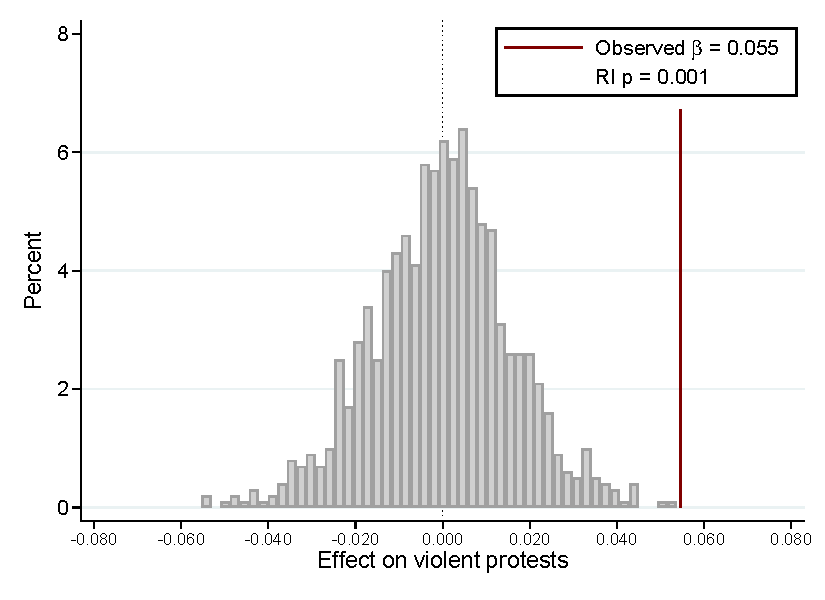
\includegraphics[width=\textwidth]{randomization_inference_hist_num_violent_MM_w30_pa.pdf}
    \end{subfigure}\hfill
    \begin{subfigure}{0.48\textwidth}
        \caption{Violent protests, $\pm 120$-day window.}
        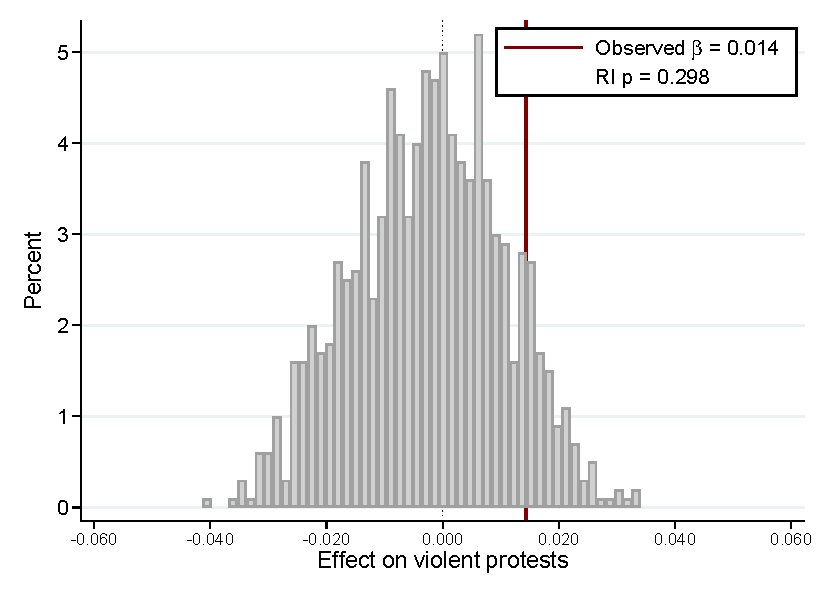
\includegraphics[width=\textwidth]{randomization_inference_hist_num_violent_MM_w120_pa.pdf}
    \end{subfigure} \\
    \begin{subfigure}{0.48\textwidth}
        \caption{Peaceful protests, $\pm 30$-day window.}
        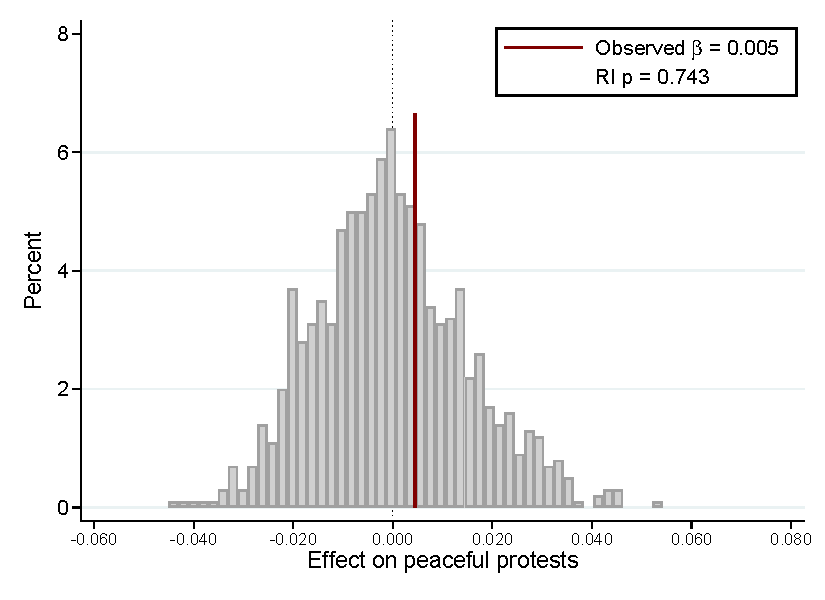
\includegraphics[width=\textwidth]{randomization_inference_hist_num_peaceful_MM_w30_pa.pdf}
    \end{subfigure}\hfill
    \begin{subfigure}{0.48\textwidth}
        \caption{Peaceful protests, $\pm 120$-day window.}
        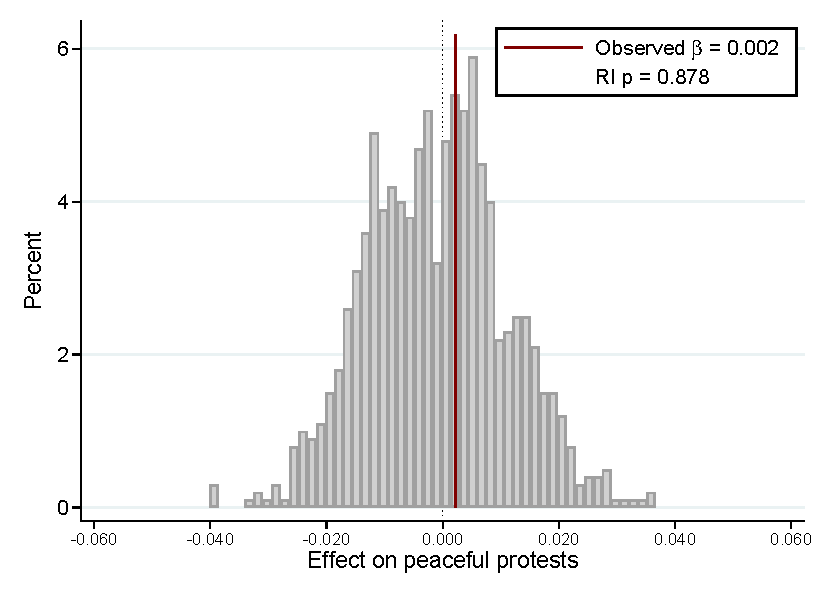
\includegraphics[width=\textwidth]{randomization_inference_hist_num_peaceful_MM_w120_pa.pdf}
    \end{subfigure}
    \footnotesize{Each histogram summarizes 1{,}000 placebo replications on the 64 scandals in the President + Other Apex subsample (Panel A of Table~\ref{tab:main}). The maroon vertical line marks the observed $\hat\beta$ from Panel A at the corresponding outcome $\times$ window cell; the top-right legend reports the two-sided randomization-inference $p$-value (share of placebo estimates with $|\hat\beta_{\mathrm{placebo}}|\geq|\hat\beta_{\mathrm{obs}}|$). Sample period 2008--2018; Venezuela excluded.}
\end{figure}

\begin{figure}[htb!]
    \caption{Randomization inference on the Other Non-Apex subsample.}
    \label{fig:sup_ri_na}
    \begin{subfigure}{0.48\textwidth}
        \caption{Violent protests, $\pm 30$-day window.}
        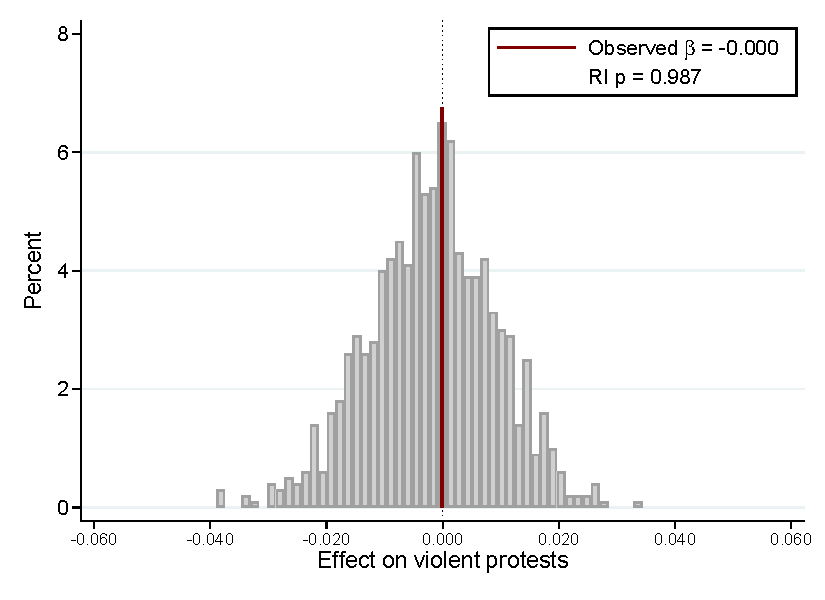
\includegraphics[width=\textwidth]{randomization_inference_hist_num_violent_MM_w30_na.pdf}
    \end{subfigure}\hfill
    \begin{subfigure}{0.48\textwidth}
        \caption{Violent protests, $\pm 120$-day window.}
        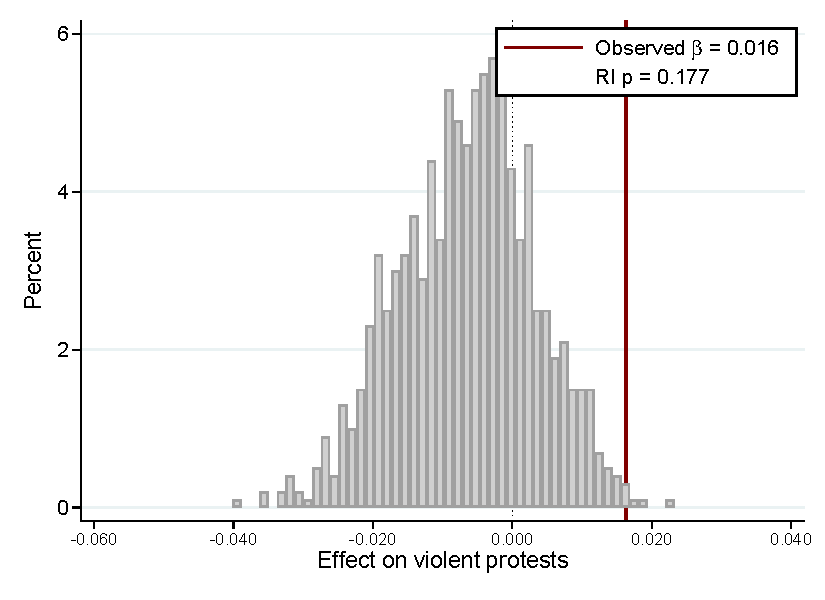
\includegraphics[width=\textwidth]{randomization_inference_hist_num_violent_MM_w120_na.pdf}
    \end{subfigure} \\
    \begin{subfigure}{0.48\textwidth}
        \caption{Peaceful protests, $\pm 30$-day window.}
        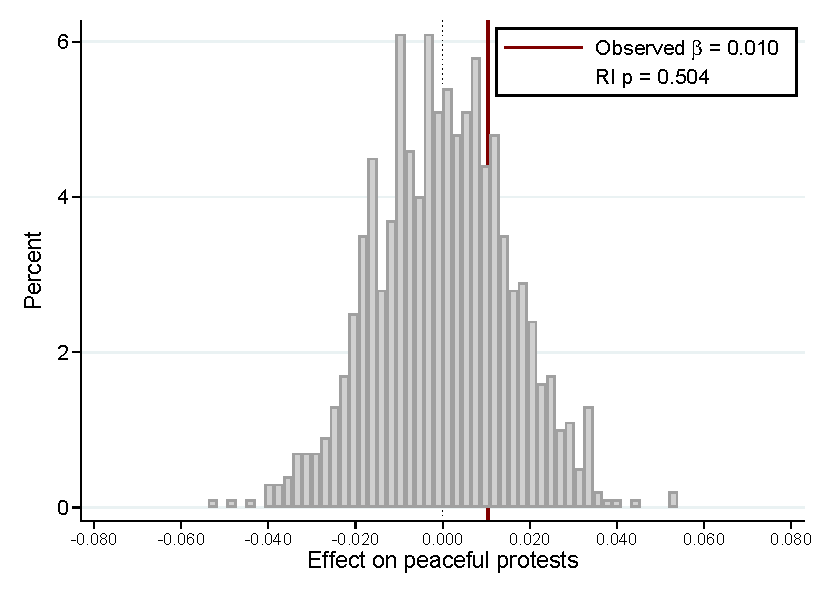
\includegraphics[width=\textwidth]{randomization_inference_hist_num_peaceful_MM_w30_na.pdf}
    \end{subfigure}\hfill
    \begin{subfigure}{0.48\textwidth}
        \caption{Peaceful protests, $\pm 120$-day window.}
        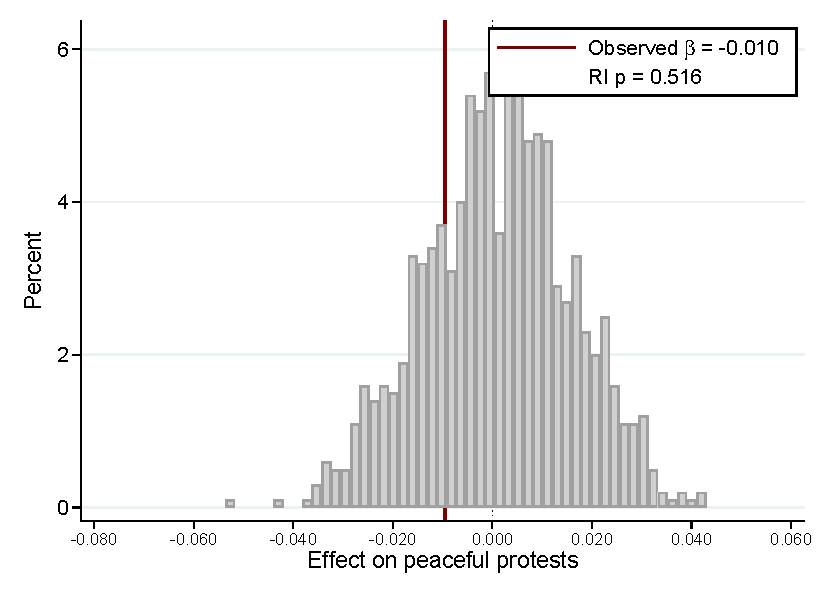
\includegraphics[width=\textwidth]{randomization_inference_hist_num_peaceful_MM_w120_na.pdf}
    \end{subfigure}
    \footnotesize{Same construction as \autoref{fig:sup_ri_pa}, restricted to the 112 scandals in the Other Non-Apex subsample (Panel B of Table~\ref{tab:main}). Sample period 2008--2018; Venezuela excluded.}
\end{figure}

% ---------------------------------------------------------------------
\clearpage
\section{Sensitivity to the event-window width}\label{sup:window}

We re-estimate the headline OLS specification at every event-window width $T \in \{15, 30, 45, \dots, 150\}$ days and plot the point estimate against $T$ with a 90\% confidence interval, separately on the President + Other Apex and Other Non-Apex subsamples. Figures~\ref{fig:sup_window_pa} and \ref{fig:sup_window_na} report the violent- and peaceful-protest panels for each subsample. Within each figure the violent and peaceful panels share a common y-axis range so the null line is aligned and magnitudes are directly comparable. The two widths reported in Table~\ref{tab:main} ($T=30$ and $T=120$) are highlighted; the effect on violent protests in the President + Other Apex subsample is positive across the full range of windows.

\begin{figure}[htb!]
    \caption{Window-width sensitivity, President + Other Apex subsample.}
    \label{fig:sup_window_pa}
    \begin{center}
    \begin{subfigure}{0.48\textwidth}
        \caption{OLS $\hat{\beta}$, violent protests.}
        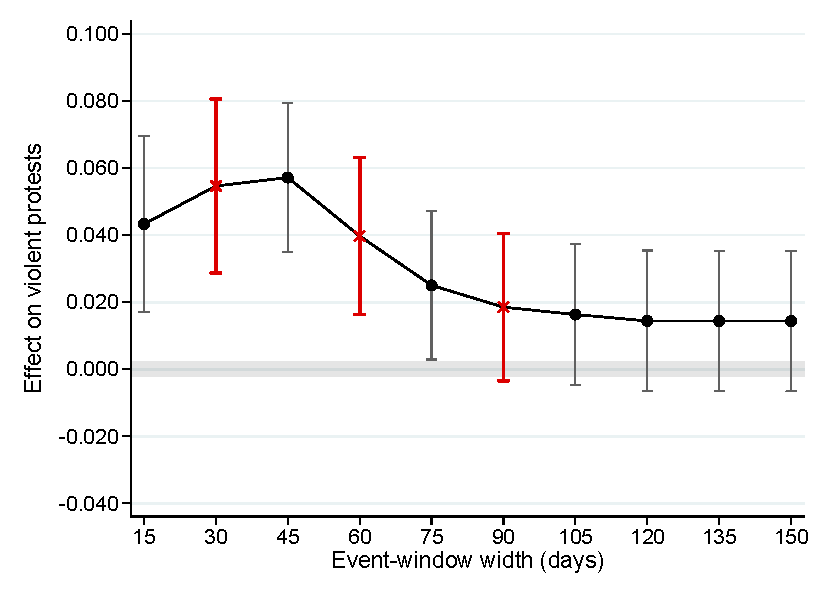
\includegraphics[width=\textwidth]{sup_window_sensitivity_ols_num_violent_MM_pa.pdf}
    \end{subfigure}\hfill
    \begin{subfigure}{0.48\textwidth}
        \caption{OLS $\hat{\beta}$, peaceful protests.}
        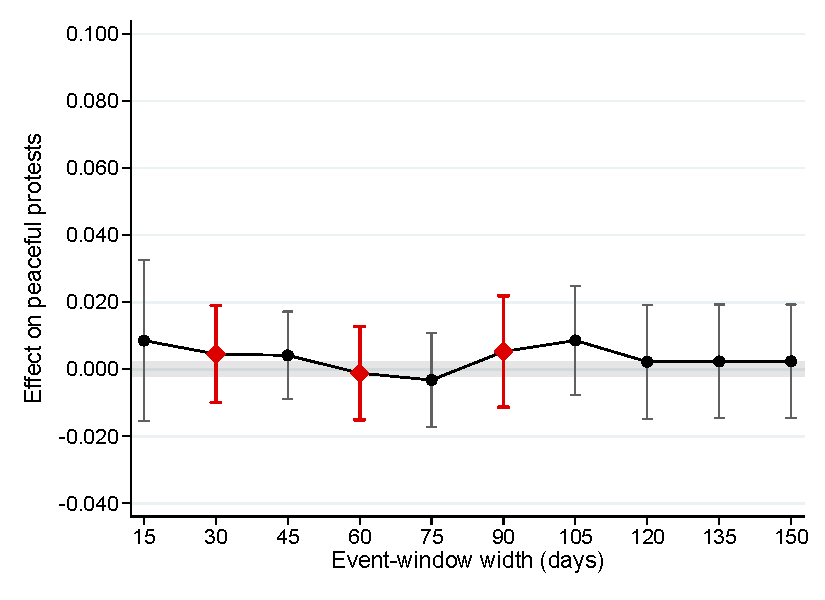
\includegraphics[width=\textwidth]{sup_window_sensitivity_ols_num_peaceful_MM_pa.pdf}
    \end{subfigure}
    \end{center}
    \footnotesize{For each $T \in \{15, 30, \dots, 150\}$ we re-estimate the headline OLS specification on the event-window panel restricted to $|w_{st}|\leq T$, on the 64 President + Other Apex scandals. Vertical bars are 90\% confidence intervals; the markers at $T=30$ and $T=120$ are highlighted. Y-axis shared between the violent and peaceful panels. Sample period 2008--2018; Venezuela excluded.}
\end{figure}

\begin{figure}[htb!]
    \caption{Window-width sensitivity, Other Non-Apex subsample.}
    \label{fig:sup_window_na}
    \begin{center}
    \begin{subfigure}{0.48\textwidth}
        \caption{OLS $\hat{\beta}$, violent protests.}
        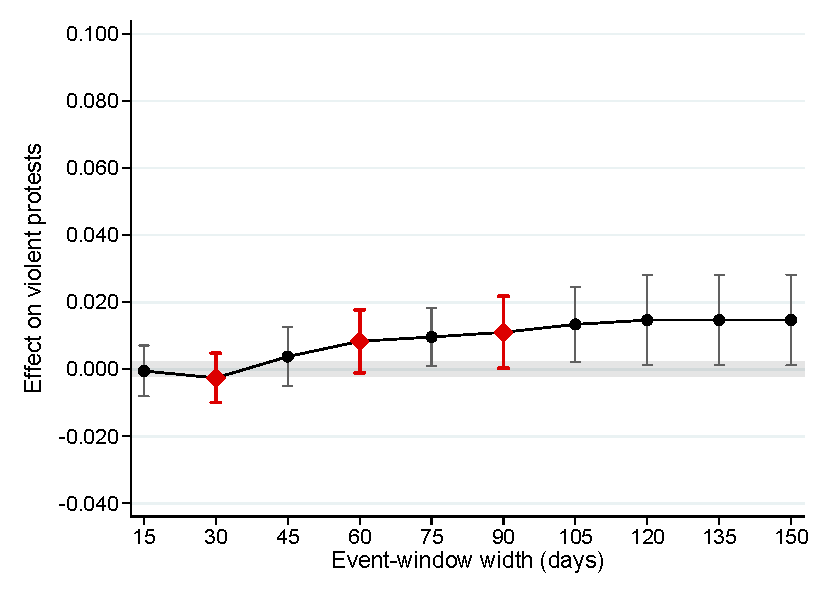
\includegraphics[width=\textwidth]{sup_window_sensitivity_ols_num_violent_MM_na.pdf}
    \end{subfigure}\hfill
    \begin{subfigure}{0.48\textwidth}
        \caption{OLS $\hat{\beta}$, peaceful protests.}
        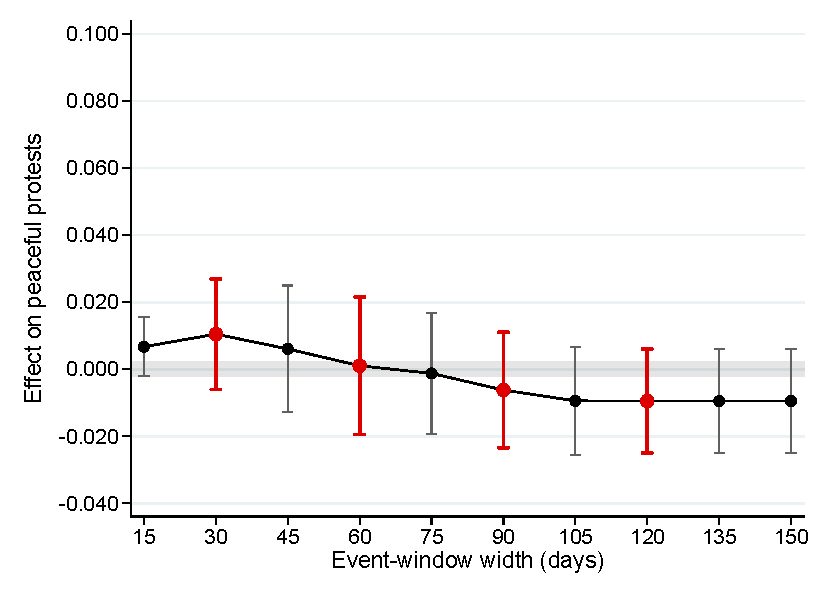
\includegraphics[width=\textwidth]{sup_window_sensitivity_ols_num_peaceful_MM_na.pdf}
    \end{subfigure}
    \end{center}
    \footnotesize{Same construction as \autoref{fig:sup_window_pa}, restricted to the 112 Other Non-Apex scandals. Y-axis shared between the violent and peaceful panels. Sample period 2008--2018; Venezuela excluded.}
\end{figure}

\end{document}
